\documentclass{article}
\usepackage[utf8]{inputenc}
\usepackage[margin=1in]{geometry} % Ajusta los márgenes a 1 pulgada
\usepackage{graphicx}
\usepackage{listings}
\usepackage{xcolor}
\usepackage{hyperref}
\usepackage{tikz}
\usepackage{biblatex}
\usepackage{lstmisc}
\usepackage{coptic}
\usetikzlibrary{shapes.multipart}

\definecolor{codegreen}{rgb}{0,0.6,0}
\definecolor{codegray}{rgb}{0.5,0.5,0.5}
\definecolor{codepurple}{rgb}{0.58,0,0.82}
\definecolor{backcolour}{rgb}{0.95,0.95,0.92}

\lstdefinestyle{mystyle}{
    backgroundcolor=\color{backcolour},
    commentstyle=\color{codegreen},
    keywordstyle=\color{magenta},
    numberstyle=\tiny\color{codegray},
    stringstyle=\color{codepurple},
    basicstyle=\ttfamily\small,
    breakatwhitespace=false,
    breaklines=true,
    captionpos=b,
    keepspaces=true,
    numbers=left,
    numbersep=5pt,
    showspaces=false,
    showstringspaces=false,
    showtabs=false,
    tabsize=2
}

\lstset{style=mystyle}

\title{Machine Learning - Lab 4 AdaBoost}
\author{RUBEN MARTINEZ GONZALEZ}
\date{Marzo 2024}

\begin{document}

    \maketitle


    \section{Introducción}\label{sec:introduccion}
    En este informe, se presenta el trabajo realizado en el laboratorio 4 de Machine Learning.
    El objetivo principal es implementar el algoritmo AdaBoost con clasificación binaria para demostrar
    cómo se puede mejorar la precisión de los clasificadores débiles al combinarlos en un modelo fuerte.
    Para entrenar el modelo que representa el algoritmo, se utilizaran los datos del archivo \texttt{dataCircle.txt}.
    Como complemento, se visualizarán las líneas de decisión de cada clasificador para una mejor comprensión de su funcionamiento.

    \noindent
    La solución se implementó en Python utilizando la biblioteca NumPy para el procesamiento de matrices y
    Matplotlib para la visualización de gráficos.
    \newline
    La implementación está desplegada en un notebook de Google Colab, el cual se puede acceder a través del siguiente enlace:
    \texttt{%
        \href{https://colab.research.google.com/drive/15pMQbVvI-XgngN3rFxADCHmMX9fd3Vl1?usp=sharing}{%
            Colab}%
    }


    \section{Implementación}\label{sec:implementacion}

    \subsection{Procesamiento de datos}\label{subsec:procesamiento_de_datos}

    Para el procesamiento de datos, se cargan los datos del archivo de texto \texttt{dataCircle.txt}
    y se extraen las primeras dos columnas como las coordenadas (x, y).
    Luego, se separan los ejemplos positivos y negativos siendo los primeros 40 ejemplos positivos y los últimos a partir del 41 ejemplos negativos.
    Finalmente, se grafican los ejemplos positivos en verde y los ejemplos negativos en rojo.

    \begin{lstlisting}[language=Python, caption={Data processing}, label={lst:data_processing}]
# Load the data from the text file
data = np.loadtxt('dataCircle.txt')

# Extract the first two columns as the x and y coordinates
x = data[:, 0]
y = data[:, 1]

# Separate the positive and negative examples
positive_examples = data[:40, :]
negative_examples = data[40:, :]

# Plot the positive examples in green
plt.scatter(positive_examples[:, 0], positive_examples[:, 1], c='g', label='Positive examples')

# Plot the negative examples in red
plt.scatter(negative_examples[:, 0], negative_examples[:, 1], c='r', label='Negative examples')

# Add labels and title
plt.xlabel('X')
plt.ylabel('Y')
plt.title('Data Plot')

# Show the plot
plt.legend()
plt.show()
    \end{lstlisting}
    Al ejecutar este bloque de código, se obtiene la siguiente gráfica:
    \begin{figure}[h]
        \centering
        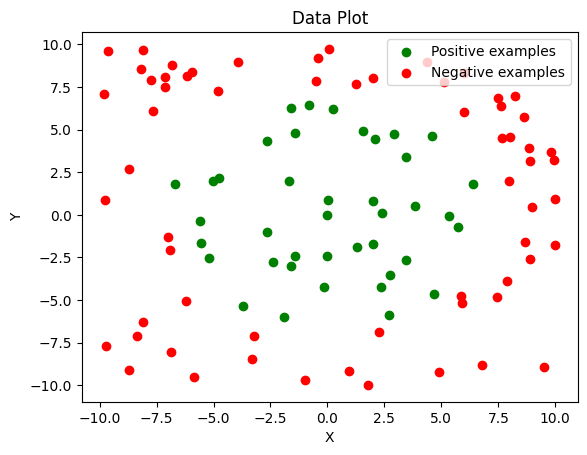
\includegraphics[width=0.5\textwidth]{img/data_plot}
        \caption{Gráfica de los datos}
        \label{fig:data_plot}
    \end{figure}

    \subsection{Implementación de AdaBoost}\label{subsec:implementacion_de_adaboost}

    Para la implementación del algoritmo, se diseñó la clase \texttt{AdaBoost} con 3 métodos principales:
    \texttt{train}, \texttt{predict} y \texttt{weak\_classifier}, y un método auxiliar \texttt{error}.
    Con estos métodos, es posible entrenar un modelo para clasificar nuevos datos
    basados en el conocimiento adquirido de los datos de entrenamiento.
    La implementación de la clase AdaBoost se describe a continuación:

    \begin{itemize}
        \item Clase AdaBoost:
        \newline
        Esta clase se inicializa recibiendo por parámetro el número de clasificadores a entrenar,
        y además, se inicializan las listas  \texttt{classifiers} y \texttt{alphas}
        que almacenarán los clasificadores débiles y los valores de $\alpha$ respectivamente.
        La clase también define los métodos \texttt{train}, \texttt{predict}, \texttt{weak\_classifier} y \texttt{compute\_error} descritos posteriormente.

        \begin{lstlisting}[language=Python, caption={AdaBoost class}, label={lst:adaboost_class}]
class AdaBoost:
    def __init__(self, n_estimators):
        self.n_estimators = n_estimators #cantidad de clasificadores
        self.alphas = []
        self.classifiers = []

    def train(self, X, y):

    def predict(self, X):

    def weak_classifier(self, X, y, D):

    def compute_error(self, y, y_pred):
        \end{lstlisting}

        \item Método train \newline
        El metodo train recibe como parámetros los datos de entrenamiento X y las etiquetas y.
        Inicializa los pesos de las muestras con 1/total para que todas las muestras igual peso y la suma quede normalizada.
        Luego, se itera sobre el número de clasificadores débiles a entrenar y para cada clasificador:
        \begin{itemize}
            \item Se encuentra el clasificador débil que minimiza el error invoca el método \texttt{weak\_classifier} descrito posteriormente.
            \item Se calcula el error del clasificador actual invocando el método \texttt{compute\_error} descrito posteriormente.
            \item Se calcula el valor de $\alpha$ del clasificador actual mediante la fórmula:
            \newline $\alpha = 0.5 * \log((1 - error) / error)$. \newline
            Este valor de $\alpha$ representará la contribución del clasificador débil al modelo final.
            \item Se agrega el clasificador actual a la lista de clasificadores y el valor de $\alpha$ a la lista de alphas.
            \item Se obtienen las predicciones del clasificador actual accediendo a la propiedad \texttt{predictions} del clasificador.
            \item Se actualizan los pesos de las muestras para que las mal clasificadas tengan más peso en las siguientes iteraciones.
            Para actualizar los pesos se almacena en la variable \texttt{weights} el resultado de multiplicar los pesos por $e^{-\alpha * y * predictions}$
            y se normalizan dividiendo por la suma de los pesos.
        \end{itemize}
        \begin{lstlisting}[language=Python, caption={train method}, label={lst:train_method}]
def train(self, X, y):
    # Inicialización de pesos
    n_samples, n_features = X.shape

    # Se inicializan los pesos de las muestras con 1/total
    weights = np.ones(n_samples) / n_samples

    for _ in range(self.n_estimators):

        # encuentra el clasificador débil que minimiza el error
        classifier = self._weak_classifier(X, y, weights)

        # calcula el error del clasificador actual
        error = self._compute_error(classifier, X, y, weights)

        # calcula alpha del clasificador actual (contribución al modelo final)
        alpha = 0.5 * np.log((1 - error) / error)

        # agrega el clasificador actual a la lista de clasificadores
        self.classifiers.append(classifier)

        # agrega el alpha del clasificador actual a la lista de alphas.
        self.alphas.append(alpha)

         # Se obtienen las predicciones del clasificador actual.
        predictions = classifier['predictions']

        #Se actualizan los pesos de las muestras
        #las muestras mal clasificadas tengan más peso en las siguientes iteraciones
        weights *= np.exp(-alpha * y * predictions)

        #Se normalizan los pesos
        weights /= np.sum(weights)
        \end{lstlisting}

        \item Método predict
        \newline
        El método predict recibe como parámetro las muestras X y retorna las predicciones finales del modelo.
        Para predecir, se inicializa un vector de ceros que contendrá las predicciones finales, y luego
        se itera sobre cada clasificador y su correspondiente $\alpha$.
        Para cada clasificador, se suman las predicciones acumuladas multiplicadas por el $\alpha$ del clasificador.
        Finalmente, si el valor es positivo, se clasifica como 1, si es negativo como -1.

        \begin{lstlisting}[language=Python, caption={predict method}, label={lst:predict_method}]
def predict(self, X):
    n_samples = X.shape[0]

    #inicializa un vector de ceros que contendrá las predicciones finales
    predictions = np.zeros(n_samples)

    #Se itera sobre cada clasificador y su correspondiente alpha
    for alpha, classifier in zip(self.alphas, self.classifiers):
        #Para cada clasificador: predicciones acumuladas = predicciones * peso
        predictions += alpha * classifier['predictions']
    #Si el valor es positivo, se clasifica como 1, si es negativo como -1
    return np.sign(predictions)
        \end{lstlisting}

        \item Método weak\_classifier
        \newline
        El método \texttt{weak\_classifier} recibe como parámetros las muestras X, las etiquetas y y los pesos de las muestras.
        Su objetivo es encontrar el clasificador débil que minimiza el error ponderado.
        Para ello, realiza la siguiente secuencia:
        \begin{itemize}
            \item Extrae el número de muestras y características del conjunto de datos.
            \item Inicializa el mejor error con infinito y el mejor clasificador con None.
            \item Itera sobre cada característica del conjunto de datos y para cada característica:
            \item Itera sobre cada valor de la característica actual como posible umbral y para cada umbral:
            \begin{itemize}
                \item Inicializa un vector de predicciones en 1 del tamaño de las muestras.
                \item Actualiza las predicciones a -1 donde el valor es menor que el umbral.
                \item Calcula el error ponderado sumando los pesos de las muestras mal clasificadas.
                \item Si el error actual es menor que el mejor error, se actualiza el mejor error y el mejor clasificador.
            \end{itemize}
            \item Retorna el mejor clasificador encontrado.
        \end{itemize}
        \begin{lstlisting}[language=Python, caption={weak\_classifier method}, label={lst:weak_classifier_method}]
def _weak_classifier(self, X, y, weights):
    n_samples, n_features = X.shape
    best_error = np.inf
    best_classifier = None
    #Itera sobre cada característica del conjunto de datos
    for feature in range(n_features):
        #Itera sobre cada valor de la característica actual como posible umbral.
        for threshold in np.unique(X[:, feature]):

            #inicializa vector de predicciones en 1.
            predictions = np.ones(n_samples)

            # actualiza las predicciones a -1 donde el valor es menor que el umbral
            predictions[X[:, feature] < threshold] = -1

            #error ponderado sumando los pesos de las muestras mal clasificadas
            error = np.sum(weights[y != predictions])

            #Si el error actual es menor, se actualiza el mejor error
            if error < best_error:
                best_error = error
                best_classifier = {'feature': feature, 'threshold': threshold, 'predictions': predictions.copy()}
    return best_classifier
        \end{lstlisting}
        \item Método error
        \newline
        El método \texttt{compute\_error} recibe como parámetros el clasificador actual, las muestras X, las etiquetas y, y los pesos de las muestras.
        Su objetivo es calcular el error ponderado del clasificador actual.
        Para ello, simplemente suma los pesos de las muestras mal clasificadas.
        \begin{lstlisting}[language=Python, caption={compute\_error method}, label={lst:compute_error_method}]
def _compute_error(self, classifier, X, y, weights):
return np.sum(weights[y != classifier['predictions']])
        \end{lstlisting}

    \end{itemize}


    \section{Entrenamiento}\label{sec:entrenamiento}
    \newline
    Para entrenar el modelo usando la clase AdaBoost, se cargan los datos del archivo \texttt{dataCircle.txt} y se separan las características y las etiquetas.
    Luego, se inicializa un objeto AdaBoost con 10 clasificadores débiles y se entrena el modelo invocando el método \texttt{train}.
    Finalmente, se realizan predicciones sobre los datos de entrenamiento y se calcula la precisión del modelo.
    Para calcular la precisión, simplemente se compara las predicciones con las etiquetas y se calcula el promedio de las coincidencias.
    Al finalizar la ejecución, se imprime en pantalla la precisión del modelo.
    \begin{lstlisting}[language=Python, caption={Training the model}, label={lst:training}]
# Load the data
data = np.loadtxt('dataCircle.txt')

# Separate features and labels
x = data[:, :2]
y = data[:, 2]

# Initialize AdaBoost with 10 weak classifiers
adaboost = AdaBoost(n_estimators=10)

# Train AdaBoost
adaboost.train(x, y)

# Make predictions
predictions = adaboost.predict(x)

# Calculate accuracy
accuracy = np.mean(predictions == y)
print("Accuracy:", accuracy)
    \end{lstlisting}


    \section{Resultados}\label{sec:resultados}
    \newline
    El ejecutar el entrenamiento del modelo, se obtiene una precisión del \texttt{0.686} lo cual está cercano a un 70\% de precisión.
    Para poder visualizar mejor el modelo, se grafican los datos de entrenamiento y las líneas de decisión de cada clasificador débil.
    Para ello, se grafican los datos de entrenamiento positivos en verde y los negativos en rojo.
    Luego, se itera sobre los clasificadores débiles y para cada clasificador:
    \begin{itemize}
        \item Se obtiene la característica y el umbral en el clasificador actual.
        \item Si la característica es 0, se grafica una línea vertical en el umbral, si no, se grafica una línea horizontal.(en ambos casos de color azul)
    \end{itemize}
Finalmente, se muestra la gráfica con los datos de entrenamiento y las líneas de decisión de los clasificadores débiles.
    \begin{lstlisting}[language=Python, caption={Plotting the decision boundaries}, label={lst:plotting}]
# Plot the positive and negative examples
plt.scatter(positive_examples[:, 0], positive_examples[:, 1], c='g', label='Positive examples')
plt.scatter(negative_examples[:, 0], negative_examples[:, 1], c='r', label='Negative examples')

#itera sobre los clasificadores débiles
for classifier in adaboost.classifiers:
# Obtiene la característica y el umbral en el clasificador actual.
feature = classifier['feature']
threshold = classifier['threshold']

# líneas de los clasificadores de color azul
if feature == 0:
plt.plot([threshold, threshold], [min(x[:, 1]), max(x[:, 1])], c='b', linestyle='--')
else:
plt.plot([min(x[:, 0]), max(x[:, 0])], [threshold, threshold], c='b', linestyle='--')

# Add labels and title
plt.xlabel('X')
plt.ylabel('Y')
plt.title('Data Plot with Weak Classifiers')

# Show the plot
plt.legend()
plt.show()
    \end{lstlisting}
    \clearpage
    Al ejecutar este bloque de código, se obtiene la siguiente gráfica:
    \begin{figure}[h]
        \centering
        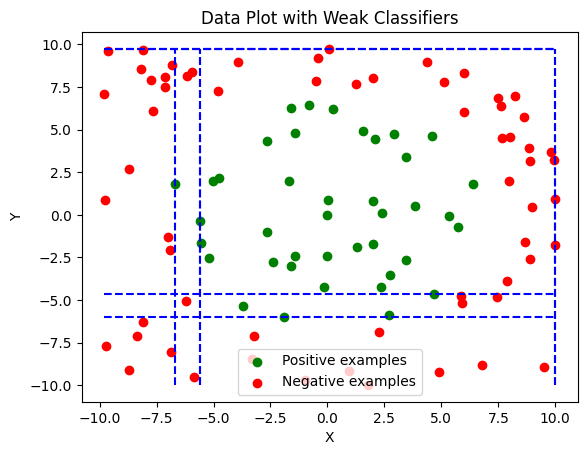
\includegraphics[width=0.5\textwidth]{img/data_plot_weak_classifiers}
        \caption{Gráfica de los datos con los clasificadores débiles}
        \label{fig:data_plot_weak_classifiers}
    \end{figure}

    \section{Conclusiones}\label{sec:conclusiones}
    \newline
    En este laboratorio, se implementó el algoritmo AdaBoost para clasificación binaria.
    Se entrenó el modelo con 10 clasificadores para los datos del archivo \texttt{dataCircle.txt} y se obtuvo una precisión del 68.6\%.
    Esto demuestra que el algoritmo AdaBoost es capaz de mejorar la precisión de los clasificadores débiles al combinarlos en un modelo fuerte.
    Además, se visualizaron las líneas de decisión de cada clasificador débil, lo que permite entender cómo se combinan para formar el modelo final.


\end{document}
